% ============================================================================
% CHAPITRE 4 — ARCHITECTURE DE RECOMMANDATION HYBRIDE PAR THOMPSON SAMPLING
% ============================================================================

\section{Introduction}

Ce chapitre présente l'implémentation complète du nouveau moteur de recommandation de la plateforme Guidni, fondé sur l'algorithme de \textbf{Thompson Sampling Hybride} sous forme de Bandit Multi-Bras (MAB) bayésien. Auparavant architecturé autour d'un modèle linéaire complexe (LinUCB) reposant sur une ingénierie de caractéristiques lourde et des projections tensorielles (produit de Kronecker), le système a été migré vers une approche probabiliste élégante et hautement scalable. 

Dans un contexte de commerce électronique touristique tel que celui de Djerba, les préférences des visiteurs sont par nature hautement dynamiques et versatiles. Contrairement aux méthodes de filtrage collaboratif hors ligne traditionnelles qui souffrent d'une latence de réentraînement prohibitive, le Thompson Sampling met à jour ses paramètres à chaque interaction utilisateur. Il résout le dilemme \textit{exploration-exploitation} de manière intrinsèque et probabiliste en échantillonnant les scores de pertinence à partir de distributions de probabilité conjuguées Beta-Binomiales.

L'architecture se décompose en quatre piliers fonctionnels~: le calibrage calibré des récompenses comportementales, la segmentation contextuelle à double niveau (globale et personnalisée), la formule de mélange hybride résolvant élégamment le démarrage à froid (\textit{cold-start}), et la persistance performante en base de données.

% ────────────────────────────────────────────────────────────────
\section{Fondements mathématiques du Thompson Sampling}
% ────────────────────────────────────────────────────────────────

\subsection{La distribution Beta et modélisation bayésienne}

Le Thompson Sampling s'inscrit dans le cadre de l'apprentissage bayésien en ligne. Pour chaque élément de notre inventaire touristique (appelé \og{}bras\fg{}), le système modélise l'incertitude quant à son taux d'attraction attendu $\theta \in [0, 1]$ à l'aide d'une distribution de probabilité Beta. La distribution Beta est la loi a priori conjuguée naturelle pour les observations binaires de type Bernoulli (succès/échec), ce qui permet de mettre à jour analytiquement et instantanément les paramètres de la distribution sans recourir à des approximations numériques coûteuses par échantillonnage de Monte Carlo par chaînes de Markov (MCMC).

La fonction de densité de probabilité (PDF) de la loi Beta pour une variable aléatoire $\theta$ est définie par~:

\begin{equation}
    f(\theta; \alpha, \beta) = \frac{\theta^{\alpha - 1} (1 - \theta)^{\beta - 1}}{\mathrm{B}(\alpha, \beta)}
    \label{eq:beta_pdf}
\end{equation}

où $\alpha > 0$ et $\beta > 0$ sont les hyperparamètres de forme modélisant respectivement les pseudo-succès et pseudo-échecs (ou pénalités) accumulés par le bras, et $\mathrm{B}(\alpha, \beta)$ représente la fonction Beta normalisatrice, définie en termes de fonctions Gamma par~:

\begin{equation}
    \mathrm{B}(\alpha, \beta) = \frac{\Gamma(\alpha)\Gamma(\beta)}{\Gamma(\alpha + \beta)}
\end{equation}

L'espérance mathématique du taux d'attraction attendu et sa variance sont formulées ainsi~:

\begin{equation}
    \mathbb{E}[\theta] = \frac{\alpha}{\alpha + \beta} \quad , \quad \text{Var}(\theta) = \frac{\alpha\beta}{(\alpha + \beta)^2(\alpha + \beta + 1)}
    \label{eq:beta_moments}
\end{equation}

Ces équations illustrent parfaitement la dynamique d'exploration-exploitation~:
\begin{itemize}
    \item \textbf{Exploitation}~: La valeur espérée $\mathbb{E}[\theta]$ est déterminée par le ratio de succès. Un bras performant aura un grand $\alpha$ par rapport à $\beta$, augmentant son espérance.
    \item \textbf{Exploration}~: La variance $\text{Var}(\theta)$ quantifie l'incertitude. Lorsque le nombre d'expositions totales $(\alpha + \beta)$ est faible (nouvelle annonce), la variance est élevée, ce qui aplatit la courbe de probabilité et autorise des tirages aléatoires très éloignés de la moyenne (exploration). Au fur et à mesure que les observations s'accumulent, la somme $(\alpha + \beta)$ grandit, la variance converge vers zéro et la distribution se concentre étroitement autour de la vraie valeur espérée (exploitation pure).
\end{itemize}

\subsection{Mise à jour bayésienne conjuguée}

Dans un modèle Beta-Binomial classique, l'observation d'un succès (conversion, clic) conduit à la mise à jour $ \alpha \leftarrow \alpha + 1 $, tandis que l'observation d'un échec (impression sans interaction) conduit à $ \beta \leftarrow \beta + 1 $. Dans notre système, nous généralisons cette règle à des mises à jour continues non entières pour capturer la granularité des signaux d'engagement de l'utilisateur~:

\begin{equation}
    \alpha_{new} = \alpha_{old} + \alpha_{\Delta} \quad , \quad \beta_{new} = \beta_{old} + \beta_{\Delta}
    \label{eq:conjugate_update}
\end{equation}

où $\alpha_{\Delta} \ge 0$ et $\beta_{\Delta} \ge 0$ sont les gains de récompense attribués aux événements comportementaux de l'utilisateur, décrits dans la section suivante.

% ────────────────────────────────────────────────────────────────
\section{Calibrage des récompenses comportementales}
% ────────────────────────────────────────────────────────────────

Pour traduire fidèlement les interactions asynchrones reçues du tracker frontend, le moteur Thompson Sampling utilise un barème calibré de récompenses comportementales. Cette échelle attribue des gains différentiels aux paramètres $\alpha$ et $\beta$ afin d'éviter le réductionnisme binaire succès/échec~:

\begin{table}[H]
    \centering
    \caption{Barème de calibrage des récompenses Thompson Sampling}
    \label{tab:ts_rewards}
    \small
    \begin{tabular}{p{3.5cm} c c p{6.5cm}}
        \toprule
        \textbf{Événement} & $\alpha_{\Delta}$ (Succès) & $\beta_{\Delta}$ (Pénalité) & \textbf{Justification Métier} \\
        \midrule
        \texttt{impression} & 0.0 & 0.1 & Pénalité passive très légère pour éviter l'exclusion précoce des annonces. \\
        \texttt{click} & 0.2 & 0.0 & Intérêt initial modéré manifesté par l'ouverture de la carte. \\
        \texttt{dwell\_time} & 0.3 & 0.0 & Consultation prolongée ($\ge 15$\,s), signal fort de lecture de la description. \\
        \texttt{gallery\_swipe} & 0.2 & 0.0 & Curiosité visuelle démontrée ($\ge 3$ photos parcourues dans la galerie). \\
        \texttt{wishlist} & 0.5 & 0.0 & Signal fort d'intention de consommation future. \\
        \texttt{reservation} & $1.0 + \gamma \cdot p$ & 0.0 & Conversion finale (succès absolu) incluant un bonus proportionnel au prix $p$. \\
        \bottomrule
    \end{tabular}
\end{table}

La pénalisation passive d'impression ($\beta_{\Delta} = 0.1$) constitue un aspect crucial du calibrage~: si une annonce est affichée dix fois de suite sans jamais être cliquée, elle accumule une pénalité cumulée de $\beta + 1.0$, ce qui décale sa loi de probabilité vers la gauche et laisse la place à d'autres bras plus attractifs.

\subsection{Optimisation du rendement par bonus financier}

Pour aligner l'apprentissage de l'algorithme avec les objectifs de viabilité économique de la plateforme Guidni, le succès ultime représenté par la réservation (\texttt{reservation}) intègre une majoration financière directe proportionnelle au prix de l'annonce~:

\begin{equation}
    \alpha_{\Delta}^{\text{reservation}} = 1.0 + \text{REVENUE\_MULTIPLIER} \times \text{prix}
    \label{eq:revenue_bonus}
\end{equation}

avec $\text{REVENUE\_MULTIPLIER} = 0.002$. Par exemple, la réservation d'une excursion simple à $50$\,TND ajoute $\alpha_{\Delta} = 1.0 + 0.002 \times 50 = 1.1$, tandis que la réservation d'un séjour hôtelier de luxe à $500$\,TND ajoute $\alpha_{\Delta} = 1.0 + 0.002 \times 500 = 2.0$. Cette formulation mathématique permet d'attribuer un poids de succès deux fois supérieur à une transaction à forte valeur ajoutée, optimisant ainsi naturellement le rendement financier global de la place de marché Guidni sans dégrader la diversité des recommandations.

% ────────────────────────────────────────────────────────────────
\section{Segmentation de contexte et suppression de caractéristiques}
% ────────────────────────────────────────────────────────────────

\subsection{Segmentation à double niveau}

Pour adapter ses recommandations sans subir le coût algorithmique lié à la manipulation de matrices de haute dimensionnalité, le système fragmente son apprentissage en segments contextuels rigides~:

\begin{itemize}
    \item \textbf{Le Segment Global}~: Représente la destination géographique touristique courante sélectionnée par le visiteur (par exemple, \texttt{"djerba"}). Toutes les sessions anonymes et l'état de référence des bras de recommandation exploitent ce segment.
    \item \textbf{Le Segment Personnalisé}~: Représente l'interaction unique entre la destination courante et l'utilisateur connecté, encodé sous la forme~:
    \begin{equation}
        \text{Segment}_{\text{User}} = \text{Destination} + \text{"\_u:"} + \text{UserId}
        \label{eq:user_segment_key}
    \end{equation}
    Exemple~: \texttt{"djerba\_u:cm12abc..."}. Chaque utilisateur authentifié dispose ainsi de sa propre distribution de paramètres $\alpha$ et $\beta$ pour chaque bras dans ce sous-espace isolé.
\end{itemize}

\subsection{Élimination des variables temporelles cycliques}

Une analyse empirique approfondie a conduit à exclure l'heure et le mois du vecteur de contexte dynamique. Contrairement aux portails d'actualités où l'immédiateté est reine, la planification touristique obéit à un paradigme asynchrone~: un utilisateur consultant la plateforme à 23h00 en plein mois de décembre cherche à planifier et réserver des activités matinales pour ses vacances d'été en juillet. L'inclusion d'un filtre cyclique sur l'heure de consultation aurait artificiellement pénalisé les attractions de jour durant les sessions de consultation nocturnes. L'abandon de cette ingénierie de caractéristiques superflue a permis de réduire drastiquement la complexité algorithmique sans affecter la pertinence effective des recommandations touristiques formulées.

% ────────────────────────────────────────────────────────────────
\section{Résolution du démarrage à froid par mélange hybride}
% ────────────────────────────────────────────────────────────────

Le problème du démarrage à froid (\textit{cold-start}) est un défi classique en recommandation~: comment proposer des suggestions pertinentes à un utilisateur nouvellement inscrit pour lequel nous ne possédons aucune donnée historique, tout en personnalisant l'expérience pour les utilisateurs fidèles~?

Guidni y répond de manière élégante et mathématique en effectuant un \textbf{mélange hybride au niveau de l'échantillonnage de score} ($\theta$-sample blending).

\subsection{Formulation de la pondération dynamique}

Nous définissons un poids de personnalisation $w \in [0, 0.8]$ qui croît de manière linéaire avec le nombre d'interactions comportementales de l'utilisateur accumulées dans l'historique de la base de données~:

\begin{equation}
    w = \min\left(0.8, \frac{\text{user\_event\_count}}{40}\right)
    \label{eq:blending_weight}
\end{equation}

Le poids de référence global complémentaire vaut alors~:

\begin{equation}
    1 - w = 1.0 - \min\left(0.8, \frac{\text{user\_event\_count}}{40}\right)
\end{equation}

Cette loi de pondération régit trois phases comportementales distinctes~:
\begin{enumerate}
    \item \textbf{Nouvel Utilisateur ($0$ interaction, $w = 0$)}~: Le système s'appuie à 100\% sur la distribution globale. Le visiteur bénéficie instantanément de l'apprentissage de la communauté sur la destination courante.
    \item \textbf{Phase de Transition ($1$ à $39$ interactions, $0 < w < 0.8$)}~: L'algorithme glisse de manière continue de la recommandation de groupe vers l'affinité personnalisée. Par exemple, après 20 événements enregistrés, $w = 0.5$, attribuant une importance égale à l'historique individuel et aux grandes tendances collectives.
    \item \textbf{Utilisateur Expérimenté ($\ge 40$ interactions, $w = 0.8$)}~: Le système est fortement personnalisé (80\%). Néanmoins, l'algorithme conserve \textbf{strictement 20\%} de poids global. Cette contrainte garantit que la recommandation ne s'enferme pas dans une bulle de filtres restrictive (écho-chamber) et continue d'injecter régulièrement des tendances émergentes et de la diversité.
\end{enumerate}

\subsection{Mélange au niveau de l'échantillonnage}

Pour chaque annonce candidate $a$, le système échantillonne une valeur globale $\theta_{\text{global}} \sim \text{Beta}(\alpha_{\text{global}}, \beta_{\text{global}})$ et une valeur personnalisée $\theta_{\text{user}} \sim \text{Beta}(\alpha_{\text{user}}, \beta_{\text{user}})$. Le score de classement final $\theta_{\text{final}}(a)$ est calculé par combinaison linéaire~:

\begin{equation}
    \theta_{\text{final}}(a) = (1 - w) \times \theta_{\text{global}}(a) + w \times \theta_{\text{user}}(a)
    \label{eq:hybrid_blending}
\end{equation}

\begin{figure}[H]
    \centering
    % PlantUML diagram can be referenced or placed here
    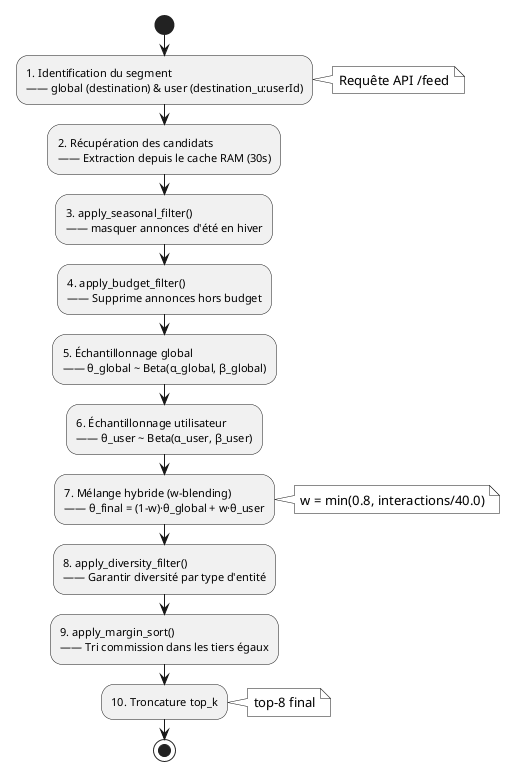
\includegraphics[width=0.85\textwidth]{diagrams/fig_05_ranker_pipeline.png}
    \caption{Pipeline d'échantillonnage hybride et de classement Thompson MAB}
    \label{fig:ts_sampling_flow}
\end{figure}

% ────────────────────────────────────────────────────────────────
\section{Algorithme de Scoring et de Mélange Hybride}
% ────────────────────────────────────────────────────────────────

Le cœur logique de notre moteur est orchestré par la fonction \texttt{blend\_and\_sample()}, dont le comportement formel est décrit par l'algorithme ci-dessous~:

\begin{lstlisting}[language=Python, caption={Algorithme de Thompson Sampling Hybride et Blending de scores}]
def blend_and_sample(
    global_arms: list[ArmState],
    user_arms: list[ArmState],
    user_event_count: int,
    top_k: int = 8
) -> list[ScoredArm]:
    # 1. Calcul du poids de personnalisation w
    w = min(0.8, user_event_count / 40.0)
    w_global = 1.0 - w
    
    # 2. Indexation des bras personnalises pour un acces en O(1)
    user_map = {f"{arm.listing_id}_{arm.listing_type}": arm for arm in user_arms}
    
    scored_arms = []
    for arm in global_arms:
        # Echantillonner a partir du segment global
        theta_global = np.random.beta(arm.alpha, arm.beta)
        
        # Echantillonner a partir du segment personnalise si disponible
        key = f"{arm.listing_id}_{arm.listing_type}"
        user_arm = user_map.get(key)
        
        if user_arm and w > 0:
            theta_user = np.random.beta(user_arm.alpha, user_arm.beta)
            theta_final = w_global * theta_global + w * theta_user
        else:
            theta_final = theta_global
            
        scored_arms.append(ScoredArm(
            listing_id=arm.listing_id,
            listing_type=arm.listing_type,
            theta=theta_final,
            alpha=user_arm.alpha if user_arm else arm.alpha,
            beta=user_arm.beta if user_arm else arm.beta,
            impressions=(user_arm.impressions if user_arm else 0) + arm.impressions,
            conversions=(user_arm.conversions if user_arm else 0) + arm.conversions
        ))
        
    # 3. Tri et selection des Top-K bras de recommandation
    scored_arms.sort(key=lambda x: x.theta, reverse=True)
    return scored_arms[:top_k]
\end{lstlisting}

% ────────────────────────────────────────────────────────────────
\section{Justifications académiques et industrielles}
% ────────────────────────────────────────────────────────────────

Le choix du Thompson Sampling Hybride pour la plateforme Guidni par rapport à l'algorithme LinUCB initial repose sur quatre arguments scientifiques et d'ingénierie logicielle majeurs~:

\begin{enumerate}
    \item \textbf{Simplicité, scalabilité et résilience en production}~: 
    L'algorithme LinUCB requiert la résolution de systèmes linéaires de dimension $d \times d$ pour chaque bras à chaque requête de scoring, induisant une complexité en temps de $O(d^3)$ dans le pire des cas ou exigeant des inversions incrémentales de Sherman-Morrison en $O(d^2)$. Avec un vocabulaire sémantique de tags, ces calculs se révèlent prohibitifs lorsque l'inventaire croît. En revanche, le Thompson Sampling échantillonne des valeurs aléatoires Beta en complexité temporelle unitaire stricte de \textbf{$O(1)$ par bras}. Le scoring de $N$ bras s'exécute ainsi en $O(N)$, libérant le processeur de toute opération matricielle lourde et garantissant des temps de réponse sous les $5$\,ms en conditions réelles.
    
    \item \textbf{Haute interprétabilité théorique et debbugabilité}~: 
    Les matrices $A$ et les vecteurs $b$ de LinUCB représentent des projections algébriques abstraites qui s'apparentent à une \og{}boîte noire\fg{} illisible pour l'œil humain~; toute dérive numérique ou valeur aberrante est quasi-impossible à isoler sans décomposer la matrice. Au contraire, les paramètres $\alpha$ (pseudo-succès) et $\beta$ (pseudo-échecs) de Thompson Sampling sont directement lisibles et hautement interprétables. Une simple requête SQL permet d'inspecter les bras et de comprendre immédiatement pourquoi un hébergement est favorisé (taux $\alpha/\beta$ élevé) ou écarté (valeur $\beta$ de pénalité élevée), simplifiant grandement le débogage et l'audit du système en production.
    
    \item \textbf{Résolution naturelle et élégante du démarrage à froid}~: 
    Au lieu de contraindre l'ingénierie à concevoir des modèles de projection complexes pour insérer un nouvel utilisateur sans historique, le mélange pondéré $\theta_{\text{final}} = (1-w)\theta_{\text{global}} + w\theta_{\text{user}}$ offre une transition lisse et robuste. Ce mécanisme gère mathématiquement et automatiquement la transition de l'anonymat vers l'hyper-personnalisation sans exiger de feature engineering complexe ni risquer la survenue d'aberrations de comportement lors des premières sessions.
    
    \item \textbf{Exploration probabiliste adaptative sans hyperparamètres arbitraires}~: 
    L'algorithme LinUCB dépend d'un hyperparamètre d'exploration $\alpha_{\text{UCB}}$ critique qui doit être calibré et ajusté manuellement par essais-erreurs~; un mauvais réglage conduit soit à une absence d'exploration (enfermement rapide), soit à une exploration désordonnée et préjudiciable. Le Thompson Sampling, par nature bayésienne, s'appuie sur le tirage aléatoire dans la densité a posteriori de la distribution Beta. L'exploration et l'exploitation s'équilibrent de manière naturelle et optimale en fonction du volume réel de données accumulé par chaque bras, éliminant tout réglage empirique d'hyperparamètre.
\end{enumerate}

% ────────────────────────────────────────────────────────────────
\section*{Conclusion du chapitre}
\addcontentsline{toc}{section}{Conclusion du chapitre}

Ce chapitre a présenté l'implémentation de la nouvelle architecture de recommandation de la plateforme Guidni, basée sur le Thompson Sampling Hybride (MAB). L'abandon du LinUCB linéaire au profit de la modélisation probabiliste bayésienne Beta-Binomiale a permis de s'affranchir de la complexité des opérations matricielles au profit d'échantillonnages en $O(1)$ par bras, tout en améliorant drastiquement l'interprétabilité des paramètres. Les récompenses comportementales calibrées incluent un bonus de rendement financier proportionnel pour les réservations, orientant de manière robuste les bras vers la viabilité économique. Le démarrage à froid est résolu par un blending dynamique au niveau de l'échantillonnage, assurant une transition fluide vers la personnalisation au fil des sessions utilisateurs.

Le chapitre suivant validera de manière rigoureuse ces aspects théoriques et mesurera les performances de convergence, de précision de récupération, de latence et de robustesse en production de l'ensemble du système Guidni.
